\section{Breakdown of costs}\label{app:cost-nodes}

\begin{figure}[H]
    \centering
    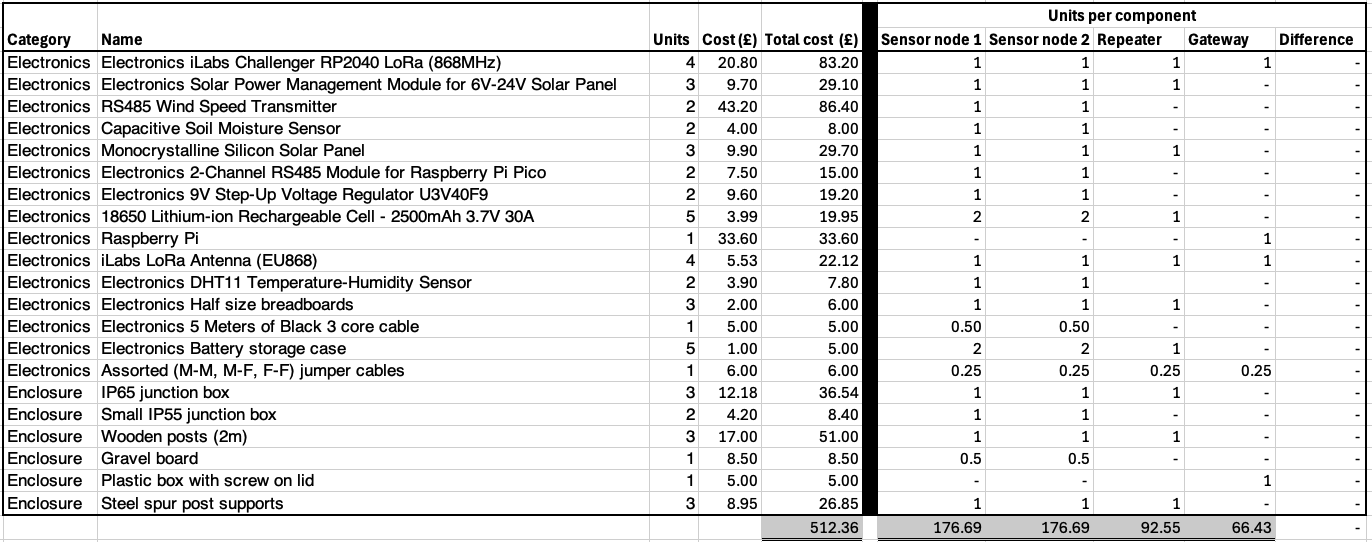
\includegraphics[width=1\textwidth]{contents/appendix/fig5/table.jpg}
    \caption{Table of component costs}
    \label{fig:cost-table}
\end{figure}

\begin{figure}[H]
    \centering
    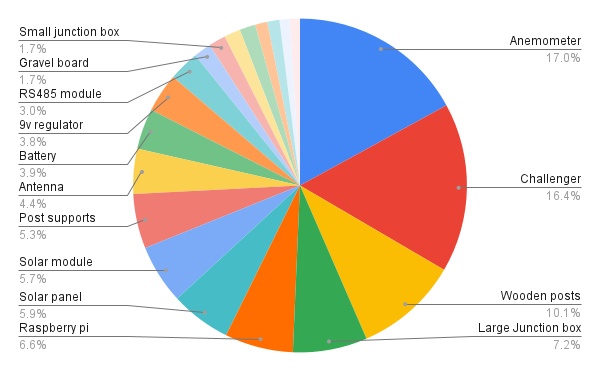
\includegraphics[width=0.8\textwidth]{contents/appendix/fig5/chart.png}
    \caption{Chart to visualise relative cost of components}
    \label{fig:cost-chart}
\end{figure}

\section{Interview excerpt with Small Brook Farms
owners}\label{sec:small-brook-interview}

Interviewer: So you would need a weather station to observe very local weather,
I expect. What you're saying is that the BBC website weather is not necessarily
relevant to you?

Speaker 1: No, No , so there's another site which is in Sanford and we can have
conversations - we're what? - 5 miles apart 10 miles? 

Speaker 2: Yeah. So the other side of that hill there like a mile away you get a
different sort of weather, but even on this side of the [apple orchard] as
opposed to that side of the [apple orchard] like the wind can be less than
whatever else, its very localised. But you know you if you then go on that side
of the valley, it doesn't rain on this side. So like to be actually useful,
yeah, [weather monitoring] sort of has to be [based on] the farm.

Source: Transcript no.28 of site visit (9 May 2025)

\section{Battery cost assumptions}\label{app:battery-assumptions}
\begin{itemize}
  \item \textbf{Agriscanner Network:} Replace 5 (2 per sensor node, 1 for
  repeater) Li-ion batteries every 3 years at a cost of \pounds{}20
  \(\Rightarrow\) \(\approx\)\,\pounds{}7 per annum.
  \item \textbf{SenseCAP S2120:} Three AA batteries per node, replaced twice a
  year (total 12 batteries) \(\approx\)\,\pounds{}10 per annum.
  \item \textbf{Decentlab Eleven Parameter:} Two C batteries per node, replaced
  four times per year (total 16 batteries) \(\approx\)\,\pounds{}30 per annum.
  \item \textbf{HOBO weather station kit:} Replace lead-acid for each node
  battery every 4 years at a cost of \pounds{}80 \(\Rightarrow\)
  \(\approx\)\,\pounds{}20 per annum.
\end{itemize}

\section{System usability survey}\label{app:sus-survey}

\begin{figure}[H]
    \centering
    
\includegraphics[width=0.9\textwidth]{contents/appendix/fig5/sus_survey.png}
    \caption{SUS survey wording}
    \label{fig:survey-wording}
\end{figure}

List of tasks for users:

\begin{enumerate}\label{list-of-tasks}
  \item To the nearest degree, what was Node 2's temperature at 14:00 18 August
  2025?
  \item To the nearest 1\,m/s, what was Node 1's gust speed at 13:00 26 August
  2025?
  \item Go to wind speed and change the graph to compare mode. What colour is
  Node 2 gusts represented by?
  \item What is the forecast for humidity at 06:00 tomorrow for Node 1?
\end{enumerate}

\section{Additional SUS materials}\label{app:correlation-sus}

\begin{figure}[H]
    \centering
    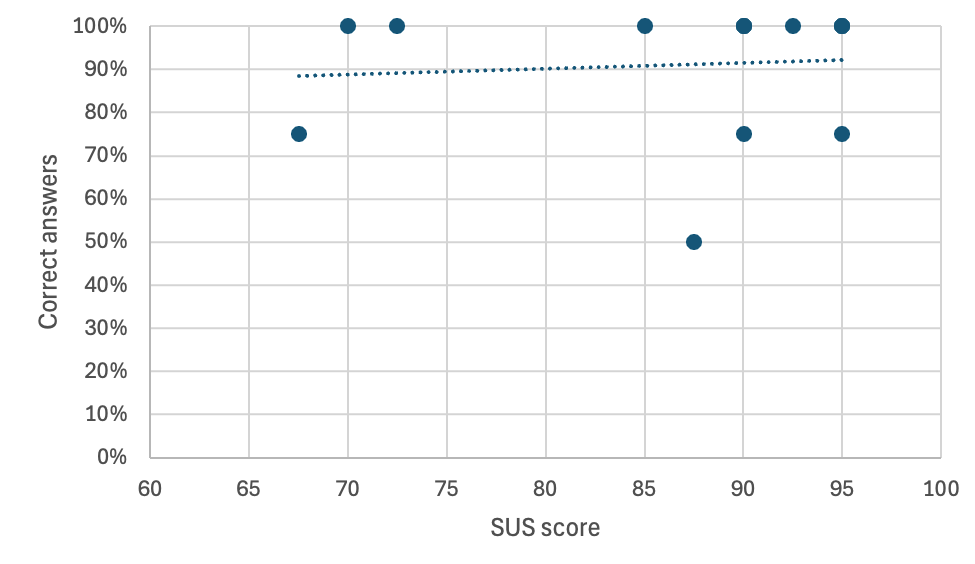
\includegraphics[width=0.9\textwidth]{contents/appendix/fig5/answer-sus-correlation.png}
    \caption{Graph to show SUS score vs percent of correct answers ($R^2 = 0.0066$)}
    \label{fig:sus-correlation}
\end{figure}

\begin{table}[ht]
  \centering
  \begin{tabular}{r r r r}
    \hline
    responder\_num & sus\_score & correct\_answers & type\\
    \hline
    1  &  90.0  & 75\%  & desktop\\
    2  &  92.5  & 100\% & mobile\\
    3  &  95.0  & 100\% & mobile\\
    4  &  70.0  & 100\% & desktop\\
    5  &  90.0  & 100\% & mobile\\
    6  &  90.0  & 100\% & desktop\\
    7  &  87.5  & 50\%  & desktop\\
    8  &  95.0  & 100\% & mobile\\
    9  &  95.0  & 75\%  & mobile\\
    10 &  95.0  & 100\% & desktop\\
    11 &  72.5  & 100\% & desktop\\
    12 &  67.5  & 75\%  & mobile\\
    13 & 100.0  & 100\% & mobile\\
    14 &  90.0  & 100\% & mobile\\
    15 &  85.0  & 100\% & desktop\\
    \hline
  \end{tabular}
  \caption{Raw SUS scores and correct answer percentage from survey}
  \label{tab:raw-sus}
\end{table}

% Requires: \usepackage{float} Also requires: \usepackage{amsmath}
\begin{figure}[H]
  \centering
  \begin{minipage}{0.9\textwidth}
    \begin{quote}
    ``I found it very hard to get to a specific time on the graph - the
    granularity of the cursor moving seemed to make it hard to choose my time -
    I ended up with 14:01 for the first question as I couldn't get the cursor to
    stay at 14:00. But as a weather nerd I loved it.''
    \end{quote}
 \vspace{8pt}
    \begin{quote}
    ``I found it annoying having to click to get to the required date. Also I
    don't understand from the website alone what the project is about or where
    the data is from - maybe an about page would be nice : )''
    \end{quote}
 \vspace{8pt}
    \begin{quote}
    ``Sorry wasn’t sure where the compare graph is but the website looked really
    nice!''
    \end{quote}
  \end{minipage}
  \caption{Feedback from participants with lower SUS scores}
  \label{fig:low-sus-feedback}
\end{figure}

\begin{figure}[H]
  \centering
  \begin{minipage}{0.9\textwidth}
    \begin{quote}
    "The soil moisture readings surprised me - I expected them to go up with
    rain (increased moisture) but they went down.  I think this is
    counter-intuitive and there should either be some explanation of the what
    the measurements mean, or preferably there should be an option to convert to
    a more human understandable description like very dry/dry/slightly
    moist.../wet/very wet/saturated"
    \end{quote}
 \vspace{8pt}
    \begin{quote}
    "When selecting the date (specifically when clicking the arrows to move
    forwards and backwards in time) it would be useful to have a calendar
    display to travel to past dates quicker."
    \end{quote}
 \vspace{8pt}
    \begin{quote}
    "Extra features: - Date picker instead of having to navigate past each day -
    Export feature to export data in bulk (e.g. to a csv) - Ability to select a
    time period (specific dates) instead of just a day view"
    \end{quote}
 \vspace{8pt}
    \begin{quote}
    "I think when switching dates, it should support selecting a date from the
    calendar rather than only moving forward or backward to the nearest dates."
    \end{quote}
 \vspace{8pt}
    \begin{quote}
    "Being able to navigate directly between measurements (e.g. temp, humidity
    etc.) while on [sic]"
    \end{quote}
 \vspace{8pt}
    \begin{quote}
    "Finding the "compare" option was the hardest part. But didn't take long." 
    \end{quote}
 \vspace{8pt}
    \begin{quote}
    "Great website- simple layout and easy to use!"
    \end{quote}
 \vspace{8pt}
    \begin{quote}
    "No bugs seen, but on wind graph some of the y axis text was slightly cut
    off on my screen. I'm on a laptop"
    \end{quote}
  \end{minipage}
  \caption{Feedback from participants with higher SUS scores}
  \label{fig:high-sus-feedback}
\end{figure}

\begin{figure}[H]
  \makebox[\textwidth][r]{ \fbox{
      \begin{minipage}[c][8cm][c]{0.85\textwidth}
        \raggedright

        Both the Mann Whitney U and Wilcoxon Signed Rank test were selected for
        this data because the SUS score is derived from Likert items. Likert
        items are ordinal (e.g. strongly disagree) and so nonparametric
        statistical testing is typically preferred
        \cite{bobbitt_mann-whitney_2022}\vspace{8pt}

    The Mann Whitney U statistical test score was calculated in an Excel sheet I
    made using the procedure described in \cite{bobbitt_mann-whitney_2022} and
    the result cross-verified using the website in \cite{socscistats} which is
    also the source of the p-value. Results: U = 13.5, critical value = 10
    p=0.10524. Parameters: two-tailed, 0.05 significance\vspace{8pt}
    
    Due to the complexity of calculating it, the one-sample Wilcoxon Signed Rank
    Test score was calculated in Excel using a modified template from the source
    in \cite{peterstatistics_wilcoxon_2025} and cross-verified with the website
    in \cite{statsBlue}. Results: \(W^{+}=119\) z = 3.3361, critical value =
    1.6449 Parameters: right-tailed, 0.05 significance \end{minipage} } }
  \caption{Note on statistical testing}
  \label{fig:appendix-note-1}
\end{figure}

\section{Nielsen's nine usability heuristics \cite{nielsen1990heuristic}}\label{app:usability-heuristics}

\begin{itemize}
  \item Simple and natural dialogue
  \item Speak the user's language
  \item Minimize user memory load
  \item Be consistent
  \item Provide feedback
  \item Provide clearly marked exits
  \item Provide shortcuts
  \item Good error messages
  \item Prevent errors
\end{itemize}

